\documentclass[12pt]{article}

% PACKAGES
\usepackage[margin = 1in]{geometry}
\usepackage{amsfonts}
\usepackage{amsmath}
\usepackage{amssymb}
\usepackage{multicol}
\usepackage{graphicx}
\usepackage{float}
\usepackage{xcolor}
\usepackage{amsthm}
\usepackage{dsfont}
\usepackage{hyperref}
\usepackage{setspace}
\usepackage{algorithm}
\usepackage{algpseudocode}

% MACROS
% Set Theory
\def\N{\mathbb{N}}
\def\R{\mathbb{R}}
\def\C{\mathbb{C}}
\def\Z{\mathbb{Z}}
%\def\^{\hat}
\def\-{\vec}
\def\d{\partial}
\def\!{\boldsymbol}
\def\X{\times}
%\def\-{\bar}
\def\bf{\textbf}
\def\l{\left}
\def\r{\right}
\def\~{\tilde}
\date{August 2022}
\doublespacing
\begin{document}

\begin{titlepage}
    \begin{center}
        \vspace*{1cm}
            
        \Huge
        \textbf{Multifidelity Finite Basis Physics Informed Neural Networks}
            
            
        \vfill
            
        
        Name: Damien Beecroft\\
        Hosting Site: Pacific Northwest National Lab\\
        Mentors: Amanda Howard and Panos Stinis\\
        \vspace{2cm}
        \begin{flushleft}
       	Mentor's Signature:\\
       	\end{flushleft}
       	\Large
        
            
    \end{center}
\end{titlepage}

\section*{Abstract}
\begin{singlespace}
Physics informed neural networks (PINNs) struggle to successfully learn solutions to differential equations that exhibit high-frequency oscillations or multi-scale behavior. Multilevel finite basis physics informed neural networks (FBPINNs) tackle this problem by recursively discretizing the solution domain and training coupled neural networks on the subdomains. High frequency structures are made less oscillatory with respect to the length scale of these smaller subdomains. This plays to the spectral bias of PINNs and enables one to learn the global solution faster. In this work we integrate multifidelity methods into multilevel FBPINNs to further improve the learning rate. This internship was virtual. I created a GitHub project to communicate what I am working on with my mentors. Anyone interested in solving differential equations could benefit from this project.
%Multifidelity PINNs are provided with both high and low fidelity data and learn the correlation between the two data sources to approximate the global solution. In the multifidelity multilevel FBPINNs framework solution approximations from previous levels supply the low fidelity data. Linear and nonlinear branch networks are then trained to learn the correlation between the low fidelity data and the true solution.\footnote{My internship was virtual, so I didn't get a chance to get any good photos!}
\end{singlespace}
\vspace{1cm}
\begin{figure}[H]
\center
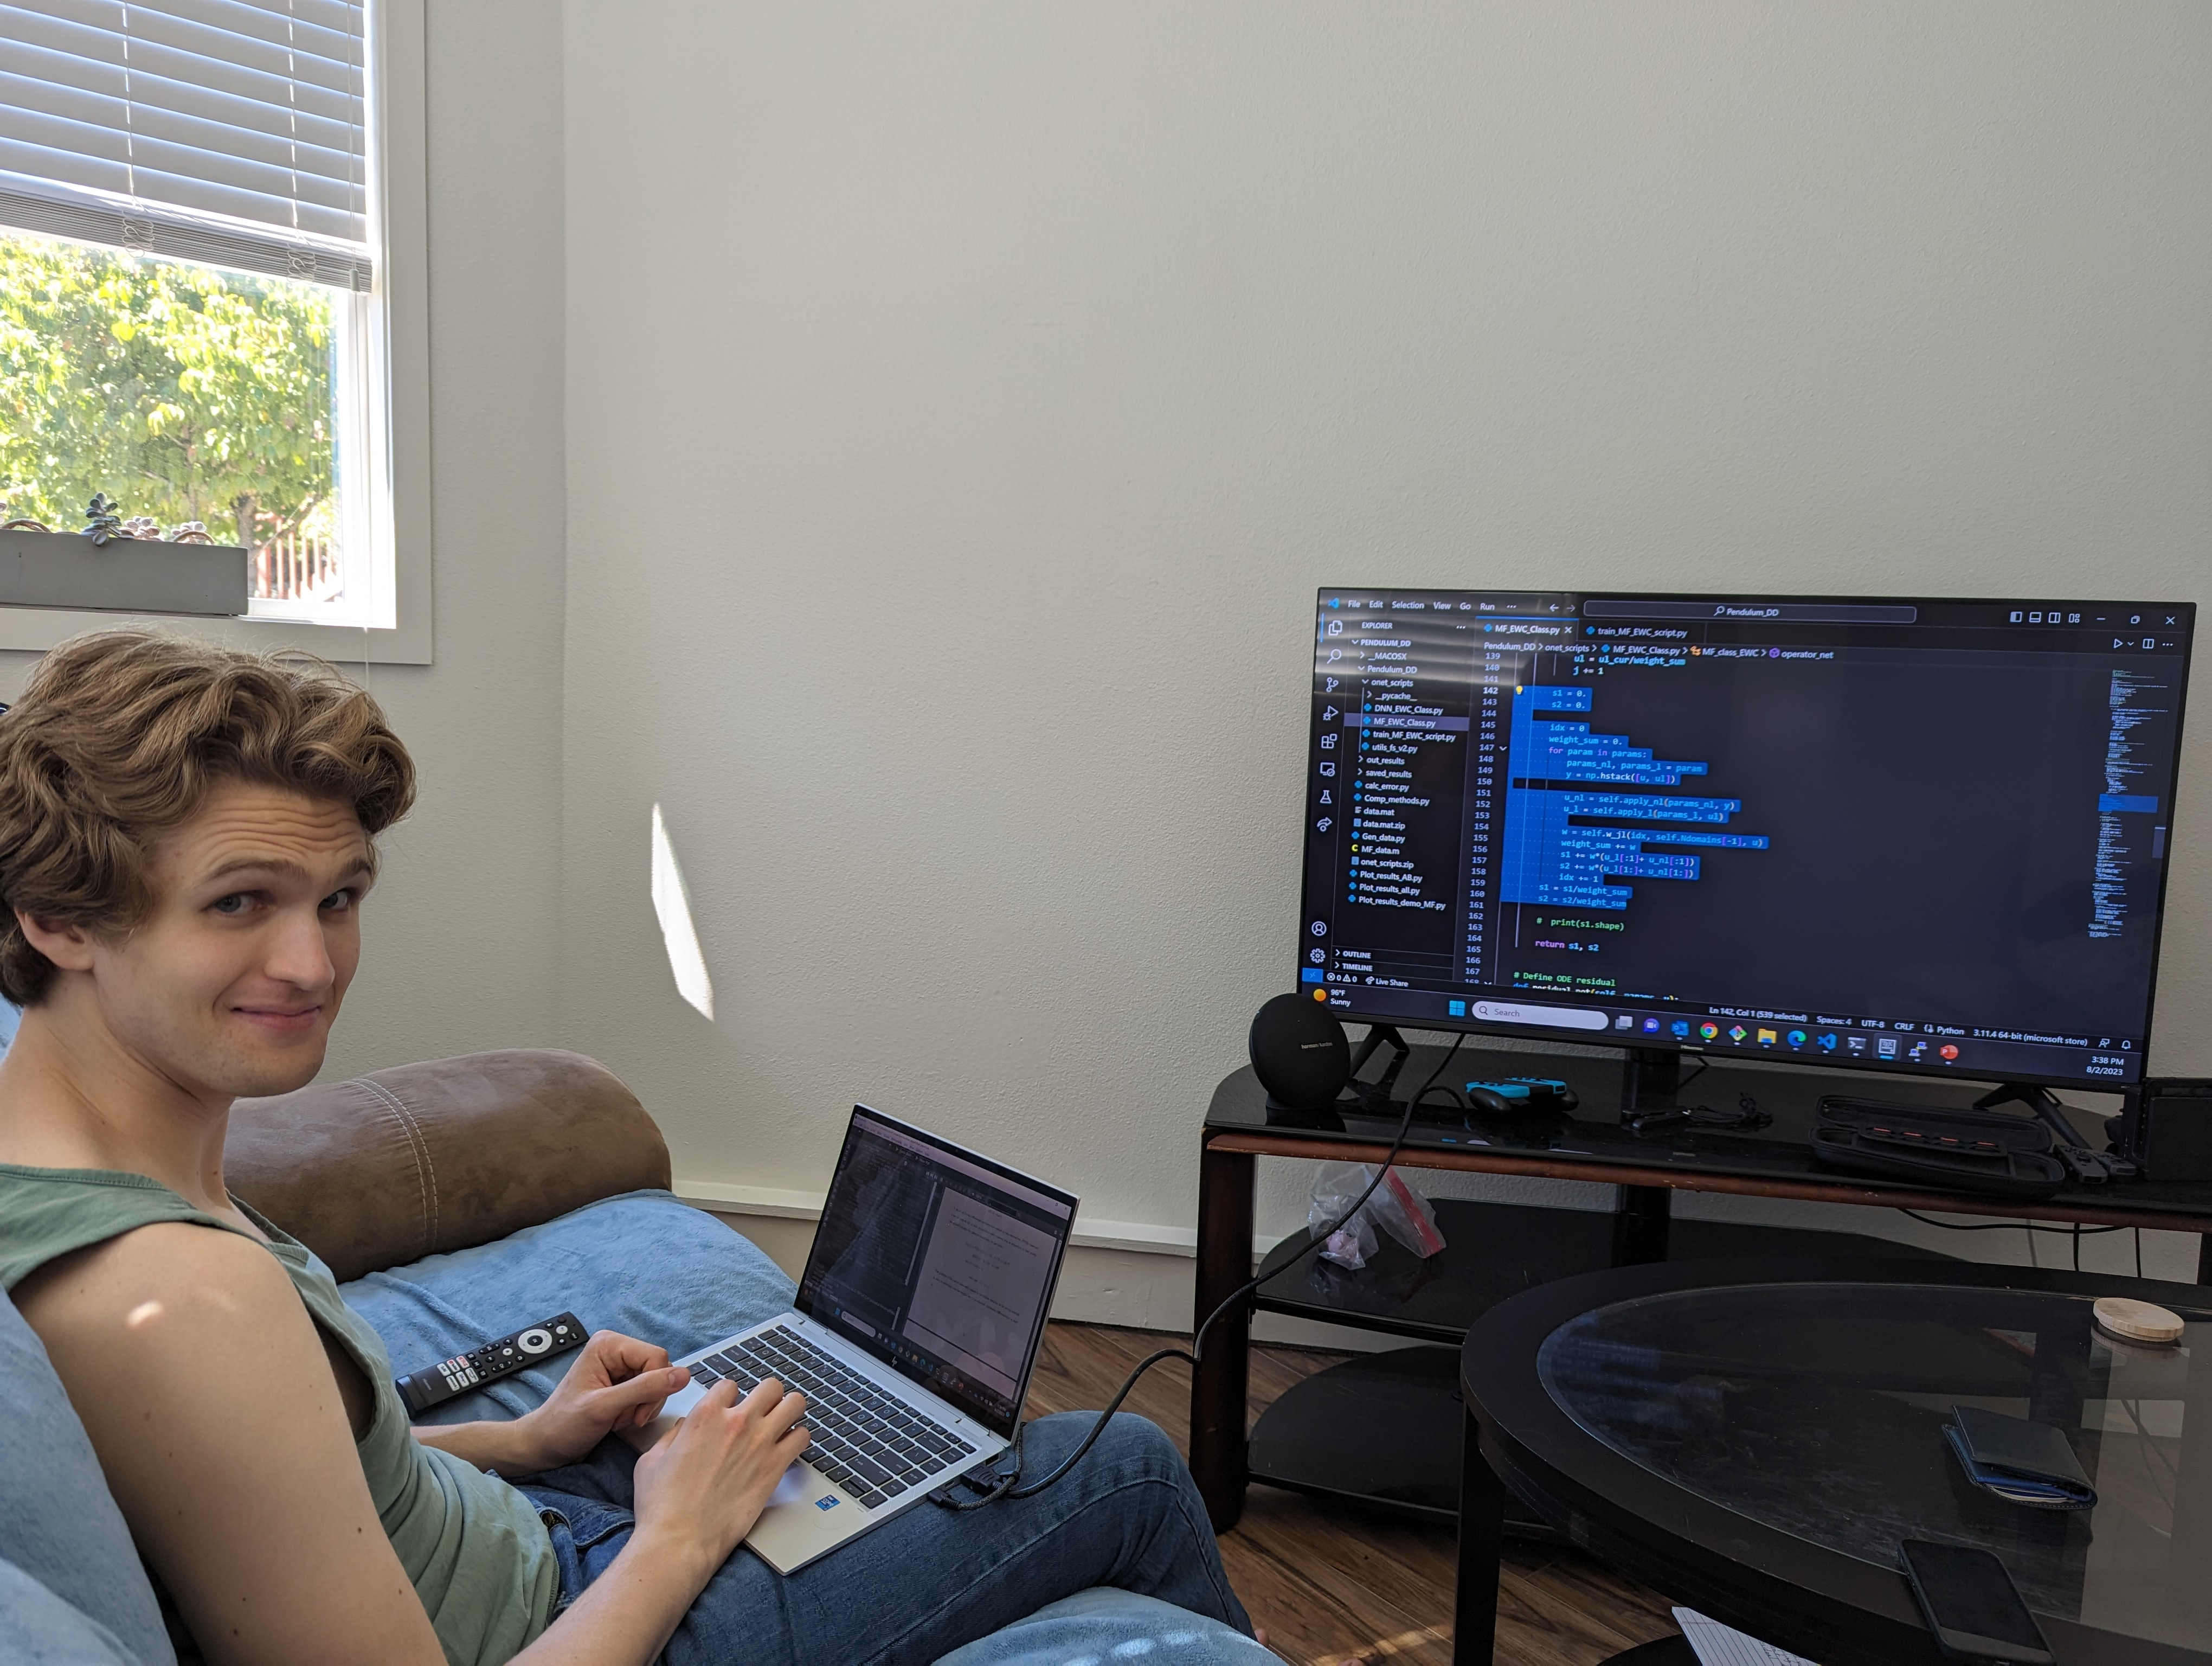
\includegraphics[width = 0.9\textwidth]{imgs/me.jpg}
\caption{My internship at Pacific Northwest National Lab was virtual. My office was anywhere I lugged my computer. On some of my more adventurous days I ventured all the way down to my living room to use the television as a secondary monitor. On an even more auspicious occasion my girlfriend and soon to be doctor Caitlin Neher was kind enough to take my photo for this final report.}
\end{figure}

\vfill
\newpage
\section{Introduction}

Raissi et al. \cite{pinns} invented the physics informed neural network (PINN) in 2016. This framework enables machine learning algorithms to learn solutions to differential equations with just the physical constraints. We briefly review the concept of a PINN here. Suppose that we have the following differential equation.
\begin{align} 
	u(t,x)_t + N[u(t,x)] &= 0 \quad \text{for} \quad x \in \Omega, \: t \in [0,T] \notag\\
	B[u(t,x)] &= 0 \quad \text{for} \quad x \in \partial \Omega\\
	u(0,x) &= u_0(x) \notag
\end{align} \label{eq:dq}
$N$ and $B$ are known differential operators that contain no time derivatives. PINNs construct a neural network $\~u(t,x)$ that, is penalized every training step in proportion to how poorly the network satisfies the physical constraints. In particular,
\begin{align*}
	\~u(t,x)_t + N[\~u(t,x)] &= l_1 \quad \text{for} \quad x \in \Omega, \: t \in [0,T];\\
	B[\~u(t,x)] &= l_2 \quad \text{for} \quad x \in \partial \Omega;\\
	\~u(0,x) - u_0(x)& = l_3;
\end{align*}
\begin{equation*}
\text{total loss} = l_1 + l_2 + l_3.
\end{equation*}
\noindent The gradient of the loss is taken with respect to the hidden variables of the neural network in order to determine how the weights are to be adjusted. Automatic differentiation is used to differentiate the neural network with respect to the temporal and spatial variables. 
\par This is a simple and elegant framework. However, PINNs struggle to learn oscillatory and multi-scale solutions, often converging to fixed point solutions of the differential equation as opposed to the true solution \cite{fixedpts}. This is often due to the fact that fixed point solutions satisfy the physical constraints of the differential equation while also maintaining small hidden weights. The boundary and initial conditions do not have enough influence to push the network away from steady state solutions. There are a variety of methods and techniques that have been introduced to improve the convergence of PINNs. Please refer to the glossary at the end for readings on some of these techniques. \textcolor{red}{MAKE GLOSSARY} 
\par My research was focused on combining two extensions of PINNs in order to help overcome the convergence difficulties. The first method is the multifidelity PINN framework introduced by Meng et al. \cite{mfpinns}. Multifidelity PINNs learn from a high and low fidelity data source. The network learns the correlation between the two data sources to achieve an accurate prediction of the true solution. The second is the multilevel finite basis PINNs as introduced in Dolean et al. \cite{fbpinns}. This construction takes the entire domain of the problem and decomposes it into a set of overlapping subdomains. A neural network is trained on each of these subdomains. My task this summer was to combine these two methods and test the performance of the resulting algorithm. The working name for this method is the Multifidelity Finite Basis Physics Informed Neural Network (MFFBPINN) algorithm. 
\par Suppose we are attempting to learn the differential equation posed in equation \ref{eq:dq}. MFFBPINNs construct a hierarchy of neural networks. On the zeroth level of the hierarchy is a single fidelity neural network that requires no low fidelity data to make a prediction. This single fidelity method could be a classical PINN or even the solution of a numerical solver. The only caveat is that we need to be able to take spatial and temporal derivatives of this single fidelity solution. After the single fidelity network is trained on $\Omega$, the domain is broken up into a set of overlapping subdomains for the first multifidelity level: $\{\Omega^1_n\}_{n=0}^{N_1}$. Each multifidelity PINN on this level takes in the evaluation of the single fidelity PINN on the zeroth level as its low fidelity approximation to the solution. Now, the multifidelity PINNs on the first level are trained while the single fidelity network's parameters are frozen. For the second level of multifidelity PINNs the process is repeated. The domain is broken up into a new set of subdomains: $\{\Omega^2_n\}_{n=0}^{N_2}$. However, now the multifidelity networks on the first level provide the low fidelity data for the second level. This process repeats until a desired accuracy is achieved.

\begin{figure}[H]
\centering
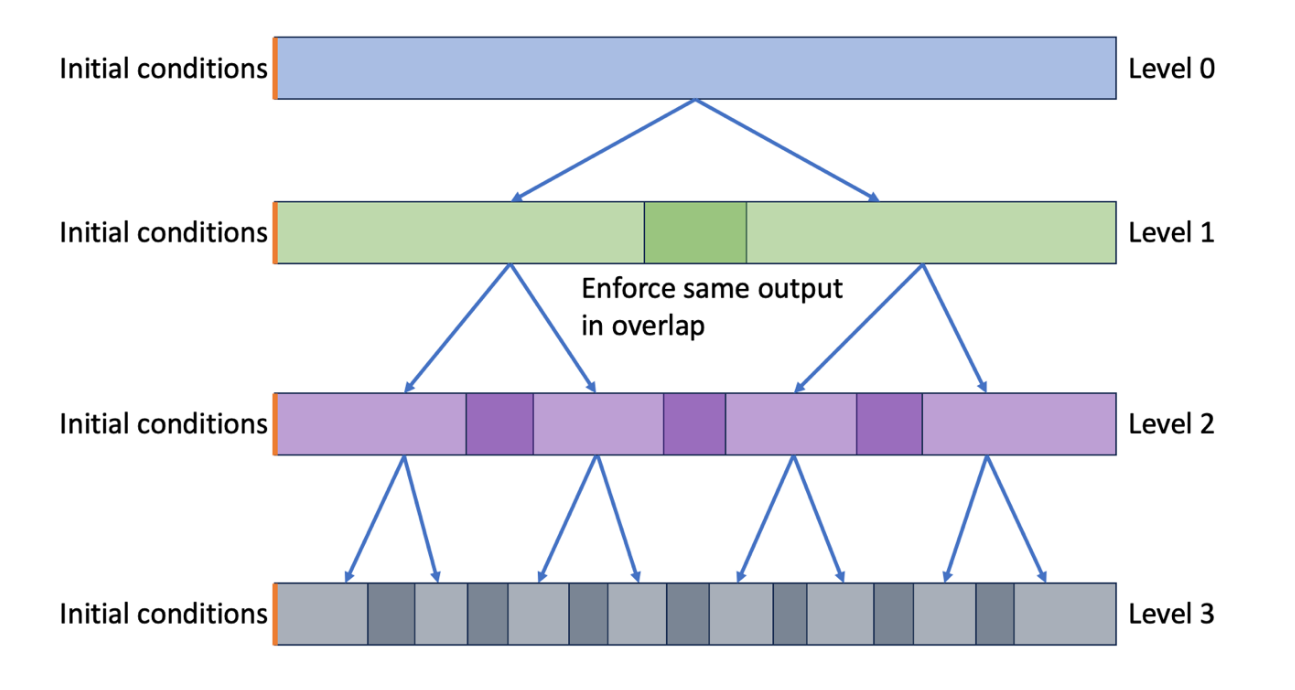
\includegraphics[width=0.7\textwidth]{imgs/domain_decomp.png}
\caption{A simple diagram of the MFFBPINN algorithm for a 1D problem where the number of domains is doubled at each step.}
\label{fig:dd}
\end{figure}

During the course of this internship, we developed two main ways to implement this algorithm. Each one is centered around how batching is done. In the first implementation, a batch containing points in the entire domain $\Omega$ is sent to the MFFBPINN. In this construction we use a tree of neural networks. The zeroth level creates its solution prediction. The networks on the first level (which are all children of the single fidelity network on the zeroth level) then look at the points in the original batch and the low fidelity solution from the zeroth layer and make their own approximation for the points that are within their subdomains. The child of each network in the second level then take in the batch points and approximations of their parents and create new approximations on the points in their subdomains and so on and so forth. A diagram illustrating this process is given in figure \ref{fig:batch1}. This method scales well with higher dimension and is rather flexible with respect to the shape of the subdomains.

\begin{figure}
\centering
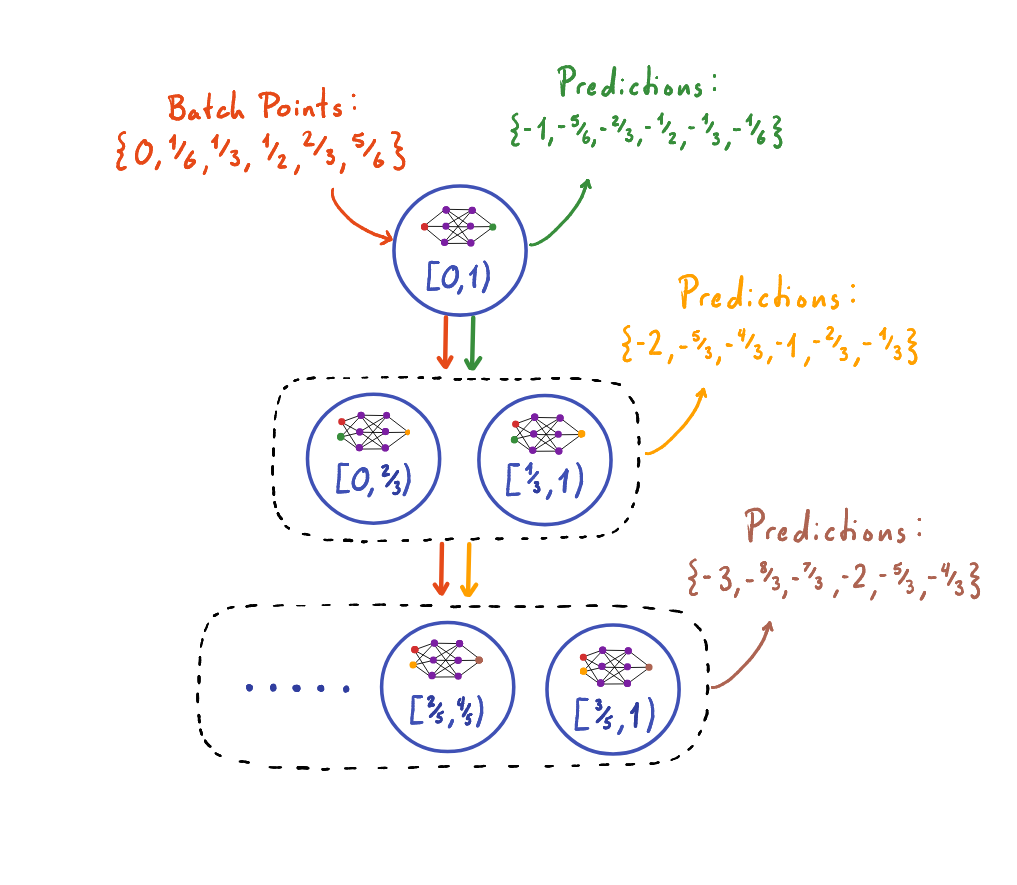
\includegraphics[width=0.7\textwidth]{imgs/batch1}
\caption{Diagram illustrating the first method for implementing the MFFBPINN.}
\label{fig:batch1}
\end{figure}

In the second implementation of the MFFBPINN, distinct batches of residual points are created for each intersection of the subdomains on the highest level. These batch points are then fed down to the neural networks on the lower levels to get the low fidelity approximations. This method is illustrated in Figure

\bibliographystyle{plain}
\bibliography{refs}
\end{document}


